\chapter{The Black Hole Information Paradox} \label{infoparadox}
Essentially the black hole information paradox arises from the fact that a quantum mechanical treatment of black holes leads to evolution of a pure initial state into a mixed state. For a pure state described by its desity matrix $\rho$, 
\begin{align}
 Tr[\rho^2] = 1
\end{align}

and using a unitary time evolution operator $U(t^\prime, t)$, 
\begin{align*}
  \rho \xrightarrow{U(t)} U \rho U^\dag
  \implies Tr[U \rho U^\dag U \rho U^\dag] = Tr[ U^\dag U \rho \rho] =  Tr[\rho^2] =1
 \end{align*}

However, consider a shell of mass $M$ in a pure state $\Ket{\psi}_M$ collapsing to form a black hole.

\begin{figure}[!h]
\centering
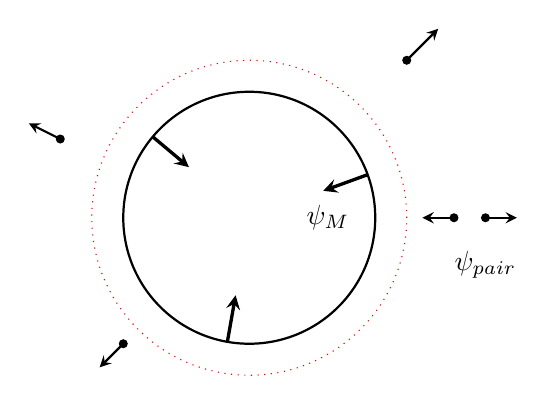
\begin{tikzpicture}[scale=2,>=stealth]
%Draw Circle radius 1 cm
    \draw[black,thick] (0,0) circle (0.8cm);
    \draw[red,dotted] (0,0) circle (1cm);
     \foreach \angle/\count in {20/1,140/2,260/3}
        {

%Draws the 3 acceleration vectors directed inward and offset slightly from the distance vectors
        \draw [name=acceleration vectors,very thick,->]
            (\angle:0.8cm) -- node[midway] {} (\angle:0.5cm) ;
    }
    \node[draw,circle,inner sep=1pt,fill] at (1,1)[] {};
    \node[draw,circle,inner sep=1pt,fill] at (1.5,0)[] {};
    \node[draw,circle,inner sep=1pt,fill] at (-1.2,0.5)[] {};
    \node[draw,circle,inner sep=1pt,fill] at (-0.8,-0.8)[] {};
    \draw [->,thick](1,1) -- (1.2,1.2);
    \draw [->,thick](1.5,0) -- (1.7,0);
    \draw [->,thick](-1.2,0.5) -- (-1.4,0.6);
    \draw [->,thick](-0.8,-0.8) -- (-0.95,-0.95);
    \node[draw=none] at (0.5,0) {$\Ket{\psi}_M$};
    
    \node[draw,circle,inner sep=1pt,fill] at (1.3,0)[] {};
    \draw [->,thick](1.3,0) -- (1.1,0);
    \node[draw=none] at (1.5,-0.3) {$\Ket{\psi}_{pair}$};
    
\end{tikzpicture}
\end{figure}

Due to the ``stretching'' of the spacelike slices, an entangled particle anti-particle pair in the sate given by:

\begin{align}
 \Ket{\psi}_\text{pair} \propto e^{\gamma c^\dag b^\dag} \Ket{0}_c \Ket{0}_b
\end{align}
Where c labels the infalling state and b labels the outgoing state. However, for qualitative purposes, it is enough to assume an entangled state of the form 
\begin{align}
 \Ket{\psi}_\text{pair} = \frac{1}{\sqrt{2}}(\Ket{0}_c \Ket{0}_b+\Ket{1}_c \Ket{1}_b)
\end{align}

The total state at this point is given (roughly) by

\begin{align}
 \Ket{\psi} \approx \Ket{\psi}_M \otimes \frac{1}{\sqrt{2}}(\Ket{0}_c \Ket{0}_b+\Ket{1}_c \Ket{1}_b)
\end{align}

and the entanglement entropy of the outgoing states (labeled by the subscript b) is given by a partial trace over the infalling state (labeled by subscript a) and the infalling mass shell M

\begin{align}
 S_b &= -Tr_{a,M}[\rho \log \rho] \\
 \implies S_b &= \log 2 
\end{align}

This $S_b$ is the entanglement (von-Neumann entropy) entropy of the subsystem b
Similarly, after propagating the timelike slice N times one ends up in the state 
\begin{align*}
 \Ket{\psi} \approx \Ket{\psi}_M &\otimes \frac{1}{\sqrt{2}}(\Ket{0}_{c1} \Ket{0}_{b1}+\Ket{1}_{c1} \Ket{1}_{b1}) \\
&\otimes \frac{1}{\sqrt{2}}(\Ket{0}_{c2} \Ket{0}_{b2}+\Ket{1}_{c2} \Ket{1}_{b2}) \\
\cdots
\end{align*}

Which gives for the entanglement entropy of the outgoing radiation
\begin{align}
 S_\text{entanglement} = N\log 2 \label{eentropy}
\end{align}

However, the outgoing radiation can be understood as thermal radiation due to the black hole radiatng away its mass. Or equivalently as the infalling particles with negative energy reducing the energy of the black hole. In either case, eventually, the black hole completely evaporates and the only remaining part is the radiated particles (system labeled by subscript b)


\begin{figure}[!h]
\centering
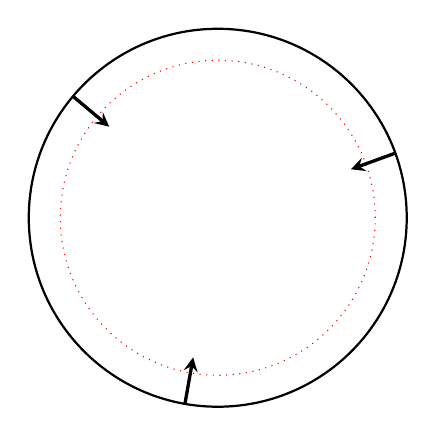
\begin{tikzpicture}[scale=2,>=stealth]
%Draw Circle radius 1 cm
    \draw[black,thick] (0,0) circle (1.2cm);
    \draw[red,dotted] (0,0) circle (1cm);
     \foreach \angle/\count in {20/1,140/2,260/3}
        {

%Draws the 3 acceleration vectors directed inward and offset slightly from the distance vectors
        \draw [name=acceleration vectors,very thick,->]
            (\angle:1.2cm) -- node[midway] {} (\angle:0.9cm) ;
    }
\end{tikzpicture}
\end{figure}



\begin{figure}[!h]
\centering
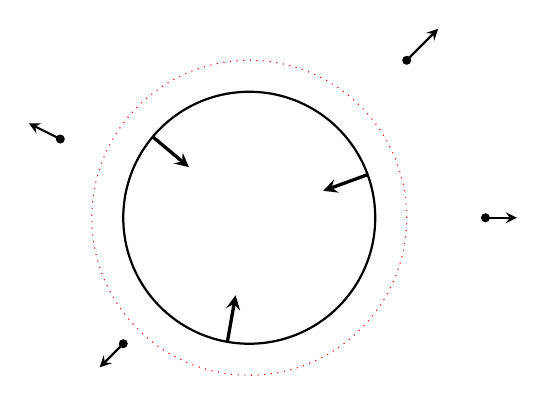
\begin{tikzpicture}[scale=2,>=stealth]
%Draw Circle radius 1 cm
    \draw[black,thick] (0,0) circle (0.8cm);
    \draw[red,dotted] (0,0) circle (1cm);
     \foreach \angle/\count in {20/1,140/2,260/3}
        {

%Draws the 3 acceleration vectors directed inward and offset slightly from the distance vectors
        \draw [name=acceleration vectors,very thick,->]
            (\angle:0.8cm) -- node[midway] {} (\angle:0.5cm) ;
    }
    \node[draw,circle,inner sep=1pt,fill] at (1,1)[] {};
    \node[draw,circle,inner sep=1pt,fill] at (1.5,0)[] {};
    \node[draw,circle,inner sep=1pt,fill] at (-1.2,0.5)[] {};
    \node[draw,circle,inner sep=1pt,fill] at (-0.8,-0.8)[] {};
    \draw [->,thick](1,1) -- (1.2,1.2);
    \draw [->,thick](1.5,0) -- (1.7,0);
    \draw [->,thick](-1.2,0.5) -- (-1.4,0.6);
    \draw [->,thick](-0.8,-0.8) -- (-0.95,-0.95);
\end{tikzpicture}
\end{figure}



\begin{figure}[!h]
\centering
\begin{tikzpicture}[scale=2,>=stealth]
%Draw Circle radius 1 cm
    \draw[black,thick] (0,0) circle (0.4cm);
    \draw[red,dotted] (0,0) circle (0.6cm);
     \foreach \angle/\count in {20/1,140/2,260/3}
        {

%Draws the 3 acceleration vectors directed inward and offset slightly from the distance vectors
        \draw [name=acceleration vectors,very thick,->]
            (\angle:0.4cm) -- node[midway] {} (\angle:0.2cm) ;
    }
    \node[draw,circle,inner sep=1pt,fill] at (1,1)[] {};
    \node[draw,circle,inner sep=1pt,fill] at (1.5,0)[] {};
    \node[draw,circle,inner sep=1pt,fill] at (-1.2,0.5)[] {};
    \node[draw,circle,inner sep=1pt,fill] at (-0.8,-0.8)[] {};
    \node[draw,circle,inner sep=1pt,fill] at (0,0.88)[] {};
    \node[draw,circle,inner sep=1pt,fill] at (0.6,-0.48)[] {};
    \draw [->,thick](1,1) -- (1.2,1.2);
    \draw [->,thick](1.5,0) -- (1.7,0);
    \draw [->,thick](-1.2,0.5) -- (-1.4,0.6);
    \draw [->,thick](-0.8,-0.8) -- (-0.95,-0.95);
    \draw [->,thick](0,0.88) -- (0,1.1);
    \draw [->,thick](0.6,-0.48) -- (0.7,-0.7);
\end{tikzpicture}
\end{figure}




\begin{figure}[!h]
\centering
\begin{tikzpicture}[scale=2,>=stealth]
%Draw Circle radius 1 cm
  
    \node[draw,circle,inner sep=1pt,fill] at (1,1)[] {};
    \node[draw,circle,inner sep=1pt,fill] at (1.5,0)[] {};
    \node[draw,circle,inner sep=1pt,fill] at (-1.2,0.5)[] {};
    \node[draw,circle,inner sep=1pt,fill] at (-0.8,-0.8)[] {};
    \node[draw,circle,inner sep=1pt,fill] at (0,0.88)[] {};
    \node[draw,circle,inner sep=1pt,fill] at (0.6,-0.48)[] {};
    \draw [->,thick](1,1) -- (1.2,1.2);
    \draw [->,thick](1.5,0) -- (1.7,0);
    \draw [->,thick](-1.2,0.5) -- (-1.4,0.6);
    \draw [->,thick](-0.8,-0.8) -- (-0.95,-0.95);
    \draw [->,thick](0,0.88) -- (0,1.1);
    \draw [->,thick](0.6,-0.48) -- (0.7,-0.7);
    
    \node[draw=none] at (0,0) {Poof!};
\end{tikzpicture}
\end{figure}


 
 
 Now, there is still a von-Neumann entropy associated with the system b given by \ref{eentropy} which is characterstic of a mixed quantum state since for a pure state we have $S=0$, and therefore to sum up, the system has evolved from a pure state to a mixed state which violates the unitarity of the time evolution operator. 
